\documentclass[paper=a4,fontsize=11pt]{scrartcl} % KOMA-article class

\usepackage{parskip}
\usepackage{graphicx}
\usepackage{caption}
\usepackage[utf8]{inputenc}
\usepackage[textwidth=17cm,textheight=25cm]{geometry}
\usepackage{amssymb,amsmath,amsthm}
\usepackage[colorlinks=true, allcolors=blue]{hyperref}

\title{Cubic spline interpolation}

\begin{document}

\maketitle
Suppose you are after a girl, and you want to impress her with your mathematical knowledge. Do some research about the 'heart curve', and we are going to do something similar - express some romantic image with a mathematical function\footnote{If the girl likes your maths function, it's probably because she already likes you, and vice versus.}. In this tutorial, I will show you how this can be done in 3 steps:

\begin{itemize}
  \item First, find an image of her favourite cartoon or anime, e.g. a portrait of Monkey·D·Luffy. Alternatively, find a figure that has a special meaning between you and her, e.g. a token of love, if you have any.
  \item Second, record some coordinates of points on the boundary of your chosen image.
  \item Third, find an mathematical curve that goes through all those points on the boundary.
\end{itemize}

The first two steps do not sound very hard, but what about the final step? Well, what we want to do is actually called interpolation. 

Consider a set of points $(x_i, y_i)$, where $x_i$ a strictly increasing sequence. We want to find a smooth curve that goes through all points $(x_i, y_i)$. Surely we can connect neighbouring points with straight line sections, but we won't get a smooth curve after all, and your girl probably won't like it too much because of those many kinks. Instead, let's connect consecutive points with cubic polynomials, and let's call those curves 'splines'.

\begin{figure}[h!]
  \centering
  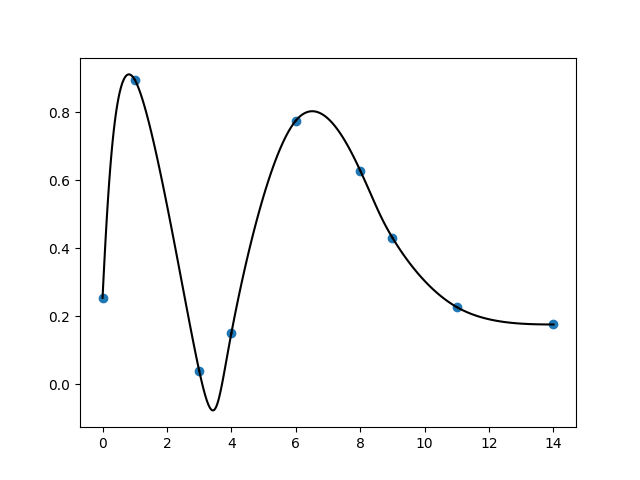
\includegraphics[width=0.5\textwidth]{random_interpolation.png}
  \caption{An example of interpolation 9 points using cubic splines.}
  \label{fig:random_interpolation}
\end{figure}

A cubic polynomial has 4 coefficients:
\begin{equation}\label{3poly}
s_i(x) = a_i + b_ix + c_ix^2 + d_ix^3.
\end{equation}
If we want to connect $N+1$ points, we need $N$ cubic polynomials, which means in total $4N$ coefficients. From high school we know that at least $4N$ equations are needed to solve for $4N$ unknowns. 

For the $i$th spline $s_i(x)$, its left and right ends must go through $(x_{i-1}, y_{i-1})$ and $(x_i, y_i)$ respectively:
\begin{equation}\label{spline_value_restriction}
\begin{split}
s_i(x_{i-1}) & = y_{i-1}, \\
s_i(x_i) & = y_{i}.
\end{split}
\end{equation}

This will contributes $2$ equations every spline, so in total $2N$ equations. In order to achieve 'smoothness', we need further restrict that the 1st and 2nd derivatives of neighbouring splines agree at the nodes:
\begin{equation}\label{spline_dev_restriction}
\begin{split}
s_i'(x_{i}) & = s_{i+1}'(x_{i}), \\
s_i''(x_{i}) & = s_{i+1}''(x_{i}).
\end{split}
\end{equation}
This condition will impose another $2N-2$ equations (why $2N-2$? Since for $N$ splines, there are only $(N-1)$ joints!). What about the last 2 equations? we can make up at the ends, e.g.:
\begin{equation}\label{derivative_end}
\begin{split}
s_1''(x_{0}) & = 0 \\
s_{N}''(x_{N}) & = 0.
\end{split}
\end{equation}
Now we have enough information to solve for those cubic polynomials. Let's start from the 2nd derivatives of splines:
\begin{equation}\label{3poly_2ndderivative}
s_i''(x) = 2 c_i + 6d_ix.
\end{equation}
The expression of $s_i''(x)$ indicates that it is a straight line connecting $(x_{i-1}, s''_{i}(x_{i-1}))$ and $(x_i, s''_i(x_{i}))$. Denote $h_i = x_i - x_{i-1}$, and $\sigma_i = s_i''(x_i)$, we obtain an expression for $s_i''(x_i)$,
\begin{equation}\label{2ndderivative_expression}
s_i''(x) = \frac{x_i - x}{h_i}\sigma_{i-1} + \frac{x - x_{i-1}}{h_i}\sigma_{i}.
\end{equation}
You can easily verify that eq.[\ref{2ndderivative_expression}] does go through $(x_{i-1}, s''_{i}(x_{i-1}))$ and $(x_i, s''_i(x_{i}))$, and is a straight line.

Next, we integrate eq.[\ref{2ndderivative_expression}] twice:
\begin{equation}\label{spline_expression}
s_i(x) = \frac{(x_i - x)^3}{6h_i}\sigma_{i-1} + \frac{(x - x_{i-1})^3}{6h_i}\sigma_{i} + \alpha_i(x-x_{i-1}) + \beta_i(x_i-x),
\end{equation}
where the last two terms are from the integration constants. Substitute eq.[\ref{spline_expression}] into eq.[\ref{spline_value_restriction}]:
\begin{equation}\label{beta}
\begin{split}
\frac{(x_i - x_{i-1})^3}{6h_i}\sigma_{i-1} + \frac{(x_{i-1} - x_{i-1})^3}{6h_i}\sigma_{i} + \alpha_i(x_{i-1}-x_{i-1}) + \beta_i(x_i-x_{i-1}) & = y_{i-1} \\
\frac{1}{6}\sigma_{i-1}h_i^2 + h_i\beta_i & = y_{i-1} \\
\beta_i & = \frac{y_{i-1}-\frac{1}{6}\sigma_{i-1}h_i^2}{h_i}
\end{split}
\end{equation}

\begin{equation}\label{alpha}
\begin{split}
\frac{(x_i - x_i)^3}{6h_i}\sigma_{i-1} + \frac{(x_i - x_{i-1})^3}{6h_i}\sigma_{i} + \alpha_i(x_i-x_{i-1}) + \beta_i(x_i-x_i) & = y_{i}\\
\frac{1}{6}\sigma_{i}h_i^2 + h_i\alpha_i & = y_{i}\\
\alpha_i & = \frac{y_{i}-\frac{1}{6}\sigma_{i}h_i^2}{h_i}.
\end{split}
\end{equation}

So far we haven't used the continuity of 1st derivatives. Integrate eq.[\ref{2ndderivative_expression}] once and substitute eq.[\ref{beta}] and eq.[\ref{alpha}],
\begin{align}\label{1stderivative_expression}
    s_i'(x) & = -\frac{(x_i - x)^2}{2h_i}\sigma_{i-1} + \frac{(x - x_{i-1})^2}{2h_i}\sigma_{i} + \alpha_i - \beta_i \\
    & = -\frac{(x_i - x)^2}{2h_i}\sigma_{i-1} + \frac{(x - x_{i-1})^2}{2h_i}\sigma_{i} + \frac{y_{i}-\frac{1}{6}\sigma_{i}h_i^2}{h_i} - \frac{y_{i-1}-\frac{1}{6}\sigma_{i-1}h_i^2}{h_i}.
\end{align}
Similarly for $s_{i+1}'(x)$:
\begin{align}\label{1stderivative_expression}
    s_{i+1}'(x) & = -\frac{(x_{i+1} - x)^2}{2h_{i+1}}\sigma_{i} + \frac{(x - x_{i})^2}{2h_{i+1}}\sigma_{i+1} + \frac{y_{i+1}-\frac{1}{6}\sigma_{i+1}h_{i+1}^2}{h_{i+1}} - \frac{y_{i}-\frac{1}{6}\sigma_{i}h_{i+1}^2}{h_{i+1}}.
\end{align}
Use the continuity of 1st derivatives $s_i'(x_{i}) = s_{i+1}'(x_{i})$, and you may skip all the algebra below...
\begin{equation}\label{1st_dev_continuity}
\begin{split}
    \frac{(x_i - x_{i-1})^2}{2h_i}\sigma_{i} + \frac{y_{i}-\frac{1}{6}\sigma_{i}h_i^2}{h_i} - \frac{y_{i-1}-\frac{1}{6}\sigma_{i-1}h_i^2}{h_i} &= -\frac{(x_{i+1} - x_i)^2}{2h_{i+1}}\sigma_{i} + \frac{y_{i+1}-\frac{1}{6}\sigma_{i+1}h_{i+1}^2}{h_{i+1}} - \frac{y_{i}-\frac{1}{6}\sigma_{i}h_{i+1}^2}{h_{i+1}}\\
    \frac{1}{2}h_i\sigma_{i} + \frac{y_{i}}{h_i}-\frac{1}{6}\sigma_{i}h_i - \frac{y_{i-1}}{h_i}+\frac{1}{6}\sigma_{i-1}h_i &= -\frac{1}{2}h_{i+1}\sigma_{i} + \frac{y_{i+1}}{h_{i+1}}-\frac{1}{6}\sigma_{i+1}h_{i+1} - \frac{y_{i}}{h_{i+1}}+\frac{1}{6}\sigma_{i}h_{i+1}\\
    3h_i\sigma_{i} -\sigma_{i}h_i +\sigma_{i-1}h_i+ 3h_{i+1}\sigma_{i} + \sigma_{i+1}h_{i+1} - \sigma_{i}h_{i+1}\ &= 6\left(\frac{y_{i+1}-y_i}{h_{i+1}}  -\frac{y_{i}-y_{i-1}}{h_i}\right)\\
    h_i\sigma_{i-1} + 2(h_{i+1}+h_i)\sigma_i+ h_{i+1}\sigma_{i+1}&=6\left(\frac{y_{i+1}-y_i}{h_{i+1}}  -\frac{y_{i}-y_{i-1}}{h_i}\right).
\end{split}
\end{equation}
Look at the final expression. This reminds us of writing it down as a matrix form $\mathbf{A}{\sigma}= \mathbf{b}$, where $\mathbf{A}$ is a tridiagonal matrix, with diagonals $2(h_{i+1}+h_i)$ and sub-diagonals $h_i$ and $h_{i+1}$. The vector $\mathbf{\sigma}$ are made of $\sigma_i$s and the vector $\mathbf{b}$ are made of $6\left(\frac{y_{i+1}-y_i}{h_{i+1}}  -\frac{y_{i}-y_{i-1}}{h_i}\right)$s. 

We then solve $\mathbf{A}{\sigma}= \mathbf{b}$ for $\mathbf{\sigma}$, and substitute $sigma$s into eq.[\ref{spline_expression}] to get our cubic splines! 

\section*{Advanced topic (challenging for pre-uni students!)}
Previously we only allow strictly increasing sequence $x_i$, which suggests that we are only able to interpolate a single-valued function $f(x_i)=y_i$. A closed curve is, however, multivalued. We must improve our method in order to interpolate a closed curve.

The theory is simple, we introduce a new parametric variable, e.g. the indices $i$ of the boundary points, which is strictly increasing. We find the cubic spline interpolations of the two sets of points $(i, x_i)$ and $(i, y_i)$ using the method above. The 0th, 1st and 2nd derivatives of $x$ w.r.t. $i$ at the nodes agree to one another, so are that for $y$. By using chain rules, the 0th, 1st and 2nd derivatives of $y$ w.r.t. $x$ also agree at nodes, which means the parametric functions $(x(i),y(i))$ are indeed cubic spline interpolation of our closed curve!

\begin{figure}[h!]
  \centering
  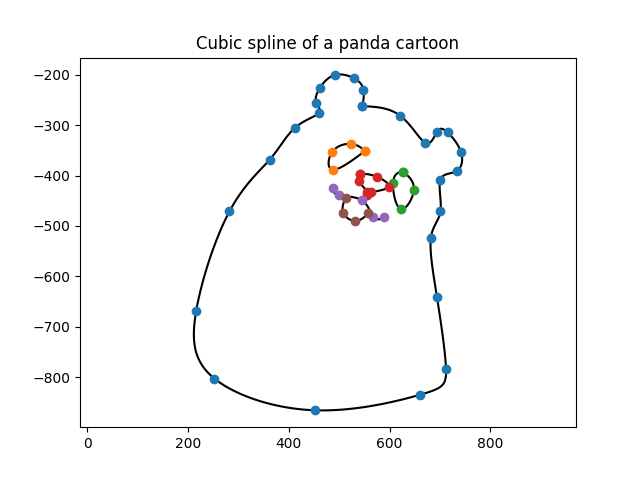
\includegraphics[width=0.5\textwidth]{interpolating_a_panda.png}
  \caption{An example of interpolation a panda cartoon.}
  \label{fig:random_interpolation}
\end{figure}


% I will show you the most basic way - pure iterations, to solve $\mathbf{A}\mathbf{\Phi}=\mathbf{b}$. There are more advanced methods to solve the equation, which are based on pure iterations, but also require a higher level understanding of linear algebra. So I will leave it later.






\end{document}
